\documentclass[border=14pt,tikz]{standalone}
\usepackage{fontspec}
\setmainfont{Helvetica Neue}
\setsansfont{Helvetica Neue}
\setmonofont{Menlo}
\usepackage{amsmath}
\usepackage{tikz}
\usetikzlibrary{positioning, arrows.meta, fit, backgrounds}

\definecolor{latent}{HTML}{E3F2FD}
\definecolor{latentborder}{HTML}{2196F3}
\definecolor{observed}{HTML}{E8F5E9}
\definecolor{observedborder}{HTML}{4CAF50}
\definecolor{weightcolor}{HTML}{E65100}

\begin{document}
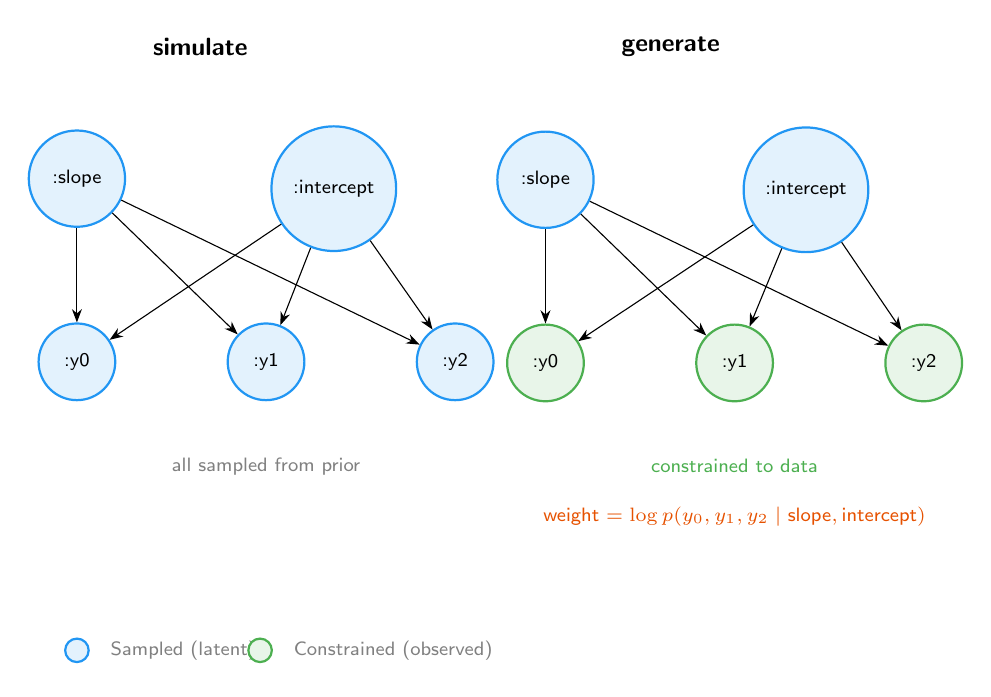
\begin{tikzpicture}[
    >=Stealth,
    node distance=1.2cm and 1.4cm,
    rv/.style={draw, circle, inner sep=6pt, font=\sffamily\scriptsize, line width=0.8pt},
    annot/.style={font=\sffamily\scriptsize, text=black!50},
    title/.style={font=\sffamily\small\bfseries},
]

% === SIMULATE ===
\node[title] (simtitle) {simulate};

\node[rv, fill=latent, draw=latentborder, below left=1cm and 0.4cm of simtitle]
    (sim-slope) {:slope};
\node[rv, fill=latent, draw=latentborder, below right=1cm and 0.4cm of simtitle]
    (sim-inter) {:intercept};

\node[rv, fill=latent, draw=latentborder, below=of sim-slope] (sim-y0) {:y0};
\node[rv, fill=latent, draw=latentborder, right=of sim-y0] (sim-y1) {:y1};
\node[rv, fill=latent, draw=latentborder, right=of sim-y1] (sim-y2) {:y2};

\draw[->] (sim-slope) -- (sim-y0);
\draw[->] (sim-slope) -- (sim-y1);
\draw[->] (sim-slope) -- (sim-y2);
\draw[->] (sim-inter) -- (sim-y0);
\draw[->] (sim-inter) -- (sim-y1);
\draw[->] (sim-inter) -- (sim-y2);

\node[annot, below=0.6cm of sim-y1] {all sampled from prior};

% === GENERATE ===
\node[title, right=4.5cm of simtitle] (gentitle) {generate};

\node[rv, fill=latent, draw=latentborder, below left=1cm and 0.4cm of gentitle]
    (gen-slope) {:slope};
\node[rv, fill=latent, draw=latentborder, below right=1cm and 0.4cm of gentitle]
    (gen-inter) {:intercept};

\node[rv, fill=observed, draw=observedborder, below=of gen-slope] (gen-y0) {:y0};
\node[rv, fill=observed, draw=observedborder, right=of gen-y0] (gen-y1) {:y1};
\node[rv, fill=observed, draw=observedborder, right=of gen-y1] (gen-y2) {:y2};

\draw[->] (gen-slope) -- (gen-y0);
\draw[->] (gen-slope) -- (gen-y1);
\draw[->] (gen-slope) -- (gen-y2);
\draw[->] (gen-inter) -- (gen-y0);
\draw[->] (gen-inter) -- (gen-y1);
\draw[->] (gen-inter) -- (gen-y2);

\node[annot, color=observedborder, below=0.6cm of gen-y1] {constrained to data};

\node[annot, color=weightcolor, below=1.2cm of gen-y1]
    {weight $= \log p(y_0, y_1, y_2 \mid \text{slope}, \text{intercept})$};

% === LEGEND ===
\node[rv, fill=latent, draw=latentborder, inner sep=3pt,
      below=3cm of sim-y0] (legL) {};
\node[annot, right=4pt of legL] {Sampled (latent)};

\node[rv, fill=observed, draw=observedborder, inner sep=3pt,
      right=2cm of legL] (legO) {};
\node[annot, right=4pt of legO] {Constrained (observed)};

\end{tikzpicture}
\end{document}
